\documentclass[letterpaper]{article}
\usepackage[top=1.0in,bottom=1.0in,left=1.0in,right=1.0in]{geometry}
\usepackage{verbatim}
\usepackage{amssymb}
\usepackage{graphicx}
\usepackage{longtable}
\usepackage{amsfonts}
\usepackage{amsmath}
\usepackage{hyperref}
\usepackage{subfigure}
\usepackage{booktabs}
\usepackage{multirow}
\usepackage[acronym,toc]{glossaries}
\hypersetup{hidelinks}
\newacronym{ANL}{ANL}{Argonne National Laboratory}
\newacronym{API}{API}{Application Programming Interface}
\newacronym{B4C}{B4C}{boron carbide}
\newacronym{BC}{BC}{boundary condition}
\newacronym{BOC}{BOC}{beginning of the equilibrium cycle}
\newacronym{BSD}{BSD}{Berkeley Software Distribution}
\newacronym{BWR}{BWR}{Boiling Water Reactor}
\newacronym{CAISO}{CAISO}{California ISO}
\newacronym{CAPP}{CAPP}{Core Analyzer for Pebble and Prism type VHTRs}
\newacronym{CEA}{CEA}{Commissariat a l'Energie Atomique}
\newacronym{CFD}{CFD}{computational fluid dynamics}
\newacronym{CO2}{CO$_2$}{carbon dioxide}
\newacronym{CR}{CR}{control rod}
\newacronym{CRP}{CRP}{Coordinated Research Project}
\newacronym{CZP}{CZP}{Cold Zero Power}
\newacronym{DCC}{DCC}{depressurized conduction cool-down}
\newacronym{DOE}{DOE}{Department of Energy}
\newacronym[\glslongpluralkey={degrees of freedom}]{DoF}{DoF}{degree of freedom}
\newacronym{EOC}{EOEC}{end of the equilibrium cycle}
\newacronym{FCEV}{FCEV}{Fuel Cell Electric Vehicle}
\newacronym{FDM}{FDM}{Finite Difference Method}
\newacronym{FEM}{FEM}{Finite Element Method}
\newacronym{FVM}{FVM}{Finite Volume Method}
\newacronym[\glslongpluralkey={greenhouse gases}]{GHG}{GHG}{greenhouse gas}
\newacronym{GRS}{GRS}{Gesellschaft für Anlagen und Reaktorsicherheit}
\newacronym{GT-MHR}{GT-MHR}{Gas Turbine-Modular Helium Reactor}
\newacronym{H2}{H$_2$}{hydrogen}
\newacronym{He}{He}{helium}
\newacronym{HFP}{HFP}{Hot Full Power}
\newacronym{HPCC}{HPCC}{high-pressure conduction cool-down}
\newacronym{HTE}{HTE}{High-Temperature Electrolysis}
\newacronym{HTGR}{HTGR}{High-Temperature Gas-Cooled Reactor}
\newacronym{HTR}{HTR}{High Temperature Reactor}
\newacronym{HTTR}{HTTR}{High-Temperature engineering Test Reactor}
\newacronym{HZDR}{HZDR}{Helmholtz-Zentrum Dresden-Rossendorf}
\newacronym{IAEA}{IAEA}{International Atomic Energy Agency}
\newacronym{icap}{iCAP}{Illinois Climate Action Plan}
\newacronym{INL}{INL}{Idaho National Laboratory}
\newacronym{IPyC}{IPyC}{inner pyrolytic carbon}
\newacronym{JFNK}{JFNK}{Jacobian-Free Newton-Krylov}
\newacronym{KAERI}{KAERI}{Korea Atomic Energy Research Institute}
\newacronym{Keff}{k$_{eff}$}{multiplication factor}
\newacronym{LBP}{LBP}{Lumped Burnable Poison}
\newacronym{LGPL}{LGPL}{Lesser GNU Public License}
\newacronym{LOCA}{LOCA}{loss of coolant accident}
\newacronym{LPCC}{LPCC}{low-pressure conduction cool-down}
\newacronym{LTE}{LTE}{Low-Temperature Electrolysis}
\newacronym{LWR}{LWR}{Light Water Reactor}
\newacronym{MC}{MC}{Monte Carlo}
\newacronym{MHTGR}{MHTGR}{Modular High-Temperature Gas-Cooled Reactor}
\newacronym{MMR}{MMR}{Micro Modular Reactor}
\newacronym{MOC}{MOC}{middle of the equilibrium cycle}
\newacronym{MOX}{MOX}{mixed-oxide}
\newacronym{MOOSE}{MOOSE}{Multi-physics Object-Oriented Simulation Environment}
\newacronym{MPI}{MPI}{Message Passing Interface}
\newacronym{MSR}{MSR}{Molten Salt Reactor}
\newacronym{MTD}{MTD}{Champaign-Urbana Mass Transit District}
\newacronym{NEA}{NEA}{Nuclear Energy Agency}
\newacronym{NEM}{NEM}{Nodal Expansion Method}
\newacronym{NGNP}{NGNP}{Next Generation Nuclear Power}
\newacronym{NRC}{NRC}{Nuclear Regulatory Commission}
\newacronym{NSC}{NSC}{Nuclear Science Committee}
\newacronym{OECD}{OECD}{Organisation for Economic Co-operation and Development}
\newacronym{OPyC}{OPyC}{outer pyrolytic carbon}
\newacronym{ORNL}{ORNL}{Oak Ridge National Laboratory}
\newacronym{OS}{OS}{Operator-Splitting}
\newacronym{PBMR}{PBMR}{Pebble Bed Modular Reactor}
\newacronym{PDE}{PDE}{Partial Differential Equation}
\newacronym{PMR}{PMR}{Prismatic Modular Reactor}
\newacronym{PV}{PV}{photovoltaics}
\newacronym{RPV}{RPV}{Reactor Pressure Vessel}
\newacronym{RSC}{RSC}{Reserve Shutdown Control}
\newacronym{RSD}{RSD}{Relative Standard Deviation}
\newacronym{SD}{SD}{Standard Deviation}
\newacronym{SI}{SI}{Sulfur-Iodine}
\newacronym{SiC}{SiC}{silicon carbide}
\newacronym{SMR}{SMR}{Small Modular Reactor}
\newacronym{SNU}{SNU}{Seoul National University}
\newacronym{SOEC}{SOEC}{Solid Oxide Electrolysis Cells}
\newacronym{SP3}{SP$_3$}{Simplified P$_3$}
\newacronym{TIP}{TIP}{transverse integration procedure}
\newacronym{TRISO}{TRISO}{Tristructural Isotropic}
\newacronym{UIUC}{UIUC}{University of Illinois at Urbana-Champaign}
\newacronym{UNIST}{UNIST}{Ulsan National Institute of Science and Technology}
\newacronym{UK}{UK}{United Kingdom}
\newacronym{UMICH}{UMICH}{University of Michigan}
\newacronym{US}{US}{United States}
\newacronym{USNC}{USNC}{Ultra Safe Nuclear Corporation}
\newacronym{VHTR}{VHTR}{Very High-Temperature Gas-Cooled Reactor}
%\newacronym{<++>}{<++>}{<++>}
%\newacronym{<++>}{<++>}{<++>}


\def\thesection       {\arabic{section}}
\def\thesubsection     {\thesection.\alph{subsection}}

\author{Roberto E. Fairhurst Agosta
        \\ \href{mailto:ref3@illinois.edu}{\texttt{ref3@illinois.edu}}
}

\title{NPRE 555\\ Computer Project 3}
\begin{document}
%\clearpage
\begin{titlepage}
\maketitle
\thispagestyle{empty}
\end{titlepage}

\section{Introduction}

For this project, I have implemented kernels in a \gls{MOOSE}-based application \cite{gaston_moose_2009} to solve the \gls{SP3} equations.
This report presents the development of those kernels as well as results of one and two-dimensional models.
Section \ref{sec:results1d} displays the results of the one-dimensional model and compares them against the results obtained with the diffusion solver in Moltres \cite{lindsay_introduction_2018}.
Section \ref{sec:results2d} presents the results of a two-dimensional model of the C5 MOX Benchmark \cite{capilla_applications_2009}.

\section{Methodology}

This section of the report introduces the followed methodology in the development of this work, comprising the following sections:
Section \ref{sec:moose} describes MOOSE framework, 
Section \ref{sec:sp3} outlines \gls{SP3} equations and their translation into kernel form,
Section \ref{sec:moltres} introduces Moltres and the equations it solves, 
and Section \ref{sec:bench} presents the C5 MOX Benchmark.

\subsection{MOOSE}
\label{sec:moose}

MOOSE is a computational framework that supports engineering analysis applications.
In a nuclear reactor, several partial differential equations describe the physical behavior.
These equations are typically nonlinear, and they are often coupled to each other.
MOOSE targets such systems and solves them in a fully coupled manner.

% more details about MOOSE
MOOSE is an open-source \gls{FEM} framework.
The framework itself relies on LibMesh \cite{kirk_libmesh_2006} and PetSc \cite{balay_petsc_2016} for solving nonlinear equations.
MOOSE applications define weak forms of the governing equations and modularize the physics expressions into "kernels."
Kernels are C++ classes containing methods for computing the residual and Jacobian contributions of individual pieces of the governing equations.
MOOSE and LibMesh translate them into residual and Jacobian functions.
These functions become inputs into PetSc solution routines.

All the software built on the MOOSE framework shares the same \gls{API}.
The applications, by default, utilize implicit methods \cite{lindsay_introduction_2018}.
This feature facilitates relatively easy coupling between different phenomena.
Additionally, the framework and its applications use \gls{MPI} for parallel communication and allow deployment on massively-parallel cluster-computing platforms.

\subsection{SP$_3$}
\label{sec:sp3}

Davidson \cite{davidson_neutron_1957} first introduced the one dimensional P$_3$ equations

\begin{align}
    & \frac{d}{dx} \phi_{1,g} + \Sigma_{t,g} \phi_{0,g} = \sum_{g'=1}^G \Sigma_{s0,g' \rightarrow g} \phi_{0,g'} + \frac{\chi_g}{k_{eff}} \sum_{g'=1}^G \nu\Sigma_{f,g'} \phi_{0,g'} + Q_{0,g}  \label{eq:SP3-0} \\
    & \frac{1}{3} \frac{d}{dx} \phi_{0,g} + \frac{2}{3}\frac{d}{dx}\phi_{2,g} + \Sigma_{t,g} \phi_{1,g} = \sum_{g'=1}^G \Sigma_{s1,g' \rightarrow g} \phi_{1,g'} + Q_{1,g} \label{eq:SP3-1} \\
    & \frac{2}{5} \frac{d}{dx}\phi_{1,g} + \frac{3}{5}\frac{d}{dx}\phi_{3,g} + \Sigma_{t,g} \phi_{2,g} = \sum_{g'=1}^G \Sigma_{s2,g' \rightarrow g} \phi_{2,g'} + Q_{2,g} \label{eq:SP3-2} \\
    & \frac{3}{7}\frac{d}{dx}\phi_{2,g} + \Sigma_{t,g} \phi_{3,g} = \sum_{g'=1}^G \Sigma_{s3,g' \rightarrow g} \phi_{3,g'} + Q_{3,g} \label{eq:P3-3} \\
    \intertext{where}
    & \phi_{n,g} = \mbox{$n^{th}$ moment of the group $g$ neutron flux } [n \cdot cm^{-2} \cdot s^{-1}]  \notag \\
    & \Sigma_{t,g} = \mbox{group $g$ macroscopic total cross-section } [cm^{-1}]  \notag \\
	& \Sigma_{sn,g' \rightarrow g} = \mbox{$n^{th}$ moment of the group $g'$ to group $g$ macroscopic scattering cross-section } [cm^{-1}]  \notag \\
	& \nu\Sigma_{f,g} = \mbox{group $g$ macroscopic production cross-section } [cm^{-1}]  \notag \\
	& \chi_{g} = \mbox{group $g$ fission spectrum } [cm^{-1}]  \notag \\
	& k_{eff} = \mbox{multiplication factor } [-]  \notag \\
	& Q_{n,g} = \mbox{$n^{th}$ group $g$ external neutron source } [n \cdot cm^{-3} \cdot s^{-1}]  \notag \\
	& G = \mbox{number of energy groups } [-].  \notag
\end{align}

Defining the group $g$ "removal" cross-section $\Sigma_{n,g}$, and assuming an isotropic external source and a negligible anisotropic group-to-group scattering \cite{brantley_simplifiedP3_2000}

\begin{align}
	& \Sigma_{n,g} = \Sigma_{t,g} - \Sigma_{sn,g' \rightarrow g} \notag \\
	& Q_{n,g} = 0, \quad n > 0 \notag \\
	& \Sigma_{sn,g' \rightarrow g} = 0, \quad g' \ne g, \quad n > 0 \notag
    \intertext{the P$_3$ equations become}
    & \frac{d}{dx} \phi_{1,g} + \Sigma_{0,g} \phi_{0,g} = \sum_{g'\ne g}^G \Sigma_{s0,g' \rightarrow g} \phi_{0,g'} + \frac{\chi_g}{k_{eff}} \sum_{g'=1}^G \nu\Sigma_{f,g'} \phi_{0,g'} + Q_{0,g}  \label{eq:SP3-0b} \\
    & \frac{1}{3} \frac{d}{dx} \phi_{0,g} + \frac{2}{3}\frac{d}{dx}\phi_{2,g} + \Sigma_{1,g} \phi_{1,g} = 0  \label{eq:SP3-1b} \\
    & \frac{2}{5} \frac{d}{dx}\phi_{1,g} + \frac{3}{5}\frac{d}{dx}\phi_{3,g} + \Sigma_{2,g} \phi_{2,g} = 0  \label{eq:SP3-2b} \\
    & \frac{3}{7}\frac{d}{dx}\phi_{2,g} + \Sigma_{3,g} \phi_{3,g} = 0. \label{eq:SP3-3b}
\end{align}

Reorganizing equations \ref{eq:SP3-1b} and \ref{eq:SP3-3b} allows for obtaining a expression for the odd moments of the flux $\phi_{1,g}$ and $\phi_{3,g}$

\begin{align}
    & \phi_{1,g} = -\frac{1}{3 \Sigma_{1,g}} \frac{d}{dx} \left[ \phi_{0,g} + 2 \phi_{2,g} \right] \label{eq:SP3-1c} \\
    & \phi_{3,g} = -\frac{3}{7 \Sigma_{3,g}}\frac{d}{dx}\phi_{2,g}. \label{eq:SP3-3c}
\end{align}

With equations \ref{eq:SP3-1c} and \ref{eq:SP3-3c}, equations \ref{eq:SP3-0b} and \ref{eq:SP3-2b} become

\begin{align}
    & - D_{0,g} \frac{d^2}{dx^2} \left( \phi_{0,g} + 2 \phi_{2,g} \right) + \Sigma_{0,g} \phi_{0,g} = \sum_{g'\ne g}^G \Sigma_{s0,g' \rightarrow g} \phi_{0,g'} + \frac{\chi_g}{k_{eff}} \sum_{g'=1}^G \nu\Sigma_{f,g'} \phi_{0,g'} + Q_{0,g}  \label{eq:SP3-0c} \\
    & - \frac{2}{5} D_{0,g} \frac{d^2}{dx^2} \left( \phi_{0,g} + 2 \phi_{2,g} \right) - D_{2,g} \frac{d^2}{dx^2} \phi_{2,g} + \Sigma_{2,g} \phi_{2,g} = 0  \label{eq:SP3-2c} \\
    \intertext{where}
    & D_{0,g} = \frac{1}{3 \Sigma_{1,g}} \notag \\
    & D_{2,g} = \frac{9}{35 \Sigma_{3,g}}. \notag
\end{align}

Introducing the variables $\Phi_{0,g}$ and $\Phi_{2,g}$ and reorganizing equations \ref{eq:SP3-0c} and \ref{eq:SP3-2c} yields

\begin{align}
    & - D_{0,g} \frac{d^2}{dx^2} \Phi_{0,g} + \Sigma_{0,g} \Phi_{0,g} - 2 \Sigma_{0,g} \Phi_{2,g} = S_{0,g} \label{eq:SP3-0d} \\
    & - D_{2,g} \frac{d^2}{dx^2} \Phi_{2,g} + \left( \Sigma_{2,g} + \frac{4}{5} \Sigma_{0,g} \right) \Phi_{2,g} - \frac{2}{5} \Sigma_{0,g} \Phi_{0,g} = -\frac{2}{5} S_{0,g} \label{eq:SP3-2d}
    \intertext{where}
    & \Phi_{0,g} = \phi_{0,g} + 2 \phi_{2,g} \notag \\
    & \Phi_{2,g} = \phi_{2,g} \notag \\
    & S_{0,g} = \sum_{g'\ne g}^G \Sigma_{s0,g' \rightarrow g} \left( \Phi_{0,g'} - 2 \Phi_{2,g'} \right) + \frac{\chi_g}{k_{eff}} \sum_{g'=1}^G \nu\Sigma_{f,g'} \left( \Phi_{0,g'} - 2 \Phi_{2,g'} \right) + Q_{0,g}. \notag
\end{align}

The $P_N$ equations yield the exact transport solution as $N \rightarrow \infty$ \cite{brantley_simplifiedP3_2000}.
In three-dimensional geometries, the number of $P_N$ equations grows like $(N+1)^2$, while in one-dimensional planar geometries, the number of equations is $(N+1)$.
The one-dimensional planar $P_N$ equations can be reformulated to yield $(N+1)/2$ coupled equations.
This realization lead Gelbard \cite{gelbard_spherical_1960} to propose the $SP_N$ approximation.
This approximation replaces the second derivatives in the one-dimensional planar $P_N$ equations with three-dimensional Laplacian operators.
This approximation yields the following equations for $N = 3$ \cite{brantley_simplifiedP3_2000}

\begin{align}
    & - D_{0,g} \Delta \Phi_{0,g} + \Sigma_{0,g} \Phi_{0,g} - 2 \Sigma_{0,g} \Phi_{2,g} = S_{0,g} \label{eq:SP3-0e} \\
    & - D_{2,g} \Delta \Phi_{2,g} + \left( \Sigma_{2,g} + \frac{4}{5} \Sigma_{0,g} \right) \Phi_{2,g} - \frac{2}{5} \Sigma_{0,g} \Phi_{0,g} = -\frac{2}{5} S_{0,g}. \label{eq:SP3-2e}
\end{align}

The Marshak vacuum \glspl{BC} complete the system of equations \cite{beckert_development_2007}

\begin{align}
    & \frac{1}{4} \Phi_{0,g} \pm \frac{1}{2} \hat{n} \cdot J_{0,g} - \frac{3}{16} \Phi_{2,g} = 0 \label{eq:SP3-BC1a} \\
    & - \frac{3}{80} \Phi_{0,g} \pm \frac{1}{2} \hat{n} \cdot J_{2,g} + \frac{21}{80} \Phi_{2,g} = 0 \label{eq:SP3-BC2a}
    \intertext{where}
    & J_{n,g} = -D_{n,g} \nabla \Phi_{n,g}. \notag
\end{align}

% advantages of SP3 over diffusion?


To define MOOSE kernels, the $SP_3$ equations are translated into weak form multiplying the equations by the test function $\Psi$ and integrating over the domain \cite{inl_workshop_2020}
\begin{align}
    & \left< \Phi, \Psi \right> = \int_V \Phi \Psi dV \\
    & \left< \Phi, \Psi \right>_{BC} = \int_S \Phi \Psi dS
    \intertext{where}
    & \Psi = \mbox{test function} \notag \\
    & V = \mbox{domain volume} \notag \\
    & S = \mbox{boundary surface}. \notag
\end{align}

The weak form of equations \ref{eq:SP3-0e} and \ref{eq:SP3-2e} becomes
\begin{align}
    & \left< - D_{0,g} \Delta \Phi_{0,g}, \Psi \right> + \left< \Sigma_{0,g} \Phi_{0,g}, \Psi \right> + \left< - 2 \Sigma_{0,g} \Phi_{2,g}, \Psi \right> + \left< - S_{0,g}, \Psi \right> = 0 \label{eq:SP3-0f} \\
    & \left< - D_{2,g} \Delta \Phi_{2,g}, \Psi \right> + \left< \left( \Sigma_{2,g} + \frac{4}{5} \Sigma_{0,g} \right) \Phi_{2,g}, \Psi \right> + \left< - \frac{2}{5} \Sigma_{0,g} \Phi_{0,g} D_{2,g}, \Psi \right> + \left< \frac{2}{5} S_{0,g}, \Psi \right> = 0. \label{eq:SP3-2f}
\end{align}

By means of Green's theorem, equations \ref{eq:SP3-0f} and \ref{eq:SP3-2f} become
\begin{align}
    & \left< D_{0,g} \nabla \Phi_{0,g}, \nabla \Psi \right> - \left< D_{0,g} \nabla \Phi_{0,g}, \Psi \right>_{BC} + \left< \Sigma_{0,g} \Phi_{0,g}, \Psi \right> + \left< - 2 \Sigma_{0,g} \Phi_{2,g}, \Psi \right> \\ &+ \left< - \sum_{g'\ne g}^G \Sigma_{s0,g' \rightarrow g} \left( \Phi_{0,g'} - 2 \Phi_{2,g'} \right), \Psi \right> + \left< - \frac{\chi_g}{k_{eff}} \sum_{g'=1}^G \nu\Sigma_{f,g'} \left( \Phi_{0,g'} - 2 \Phi_{2,g'} \right), \Psi \right> + \left< - Q_{0,g}, \Psi \right> = 0 \label{eq:SP3-0g} \\
    & \left< D_{2,g} \nabla \Phi_{2,g}, \nabla \Psi \right> - \left< D_{2,g} \nabla \Phi_{2,g}, \Psi \right>_{BC} + \left< \left( \Sigma_{2,g} + \frac{4}{5} \Sigma_{0,g} \right) \Phi_{2,g}, \Psi \right> + \left< - \frac{2}{5} \Sigma_{0,g} \Phi_{0,g}, \Psi \right> \\ &+ \left< \frac{2}{5} \sum_{g'\ne g}^G \Sigma_{s0,g' \rightarrow g} \left( \Phi_{0,g'} - 2 \Phi_{2,g'} \right), \Psi \right> + \left< \frac{2}{5} \frac{\chi_g}{k_{eff}} \sum_{g'=1}^G \nu\Sigma_{f,g'} \left( \Phi_{0,g'} - 2 \Phi_{2,g'} \right), \Psi \right> + \left< \frac{2}{5} Q_{0,g}, \Psi \right> = 0. \label{eq:SP3-2g}
    \intertext{where the boundary condition terms come from the translation into weak form of equations \ref{eq:SP3-BC1a} and \ref{eq:SP3-BC2a}, giving}
    & \left< D_{0,g} \nabla \Phi_{0,g}, \Psi \right>_{BC} = \left< \frac{1}{2} \Phi_{0,g} - \frac{3}{4} \Phi_{2,g}, \Psi \right>_{BC} \\
    & \left< D_{2,g} \nabla \Phi_{2,g}, \Psi \right>_{BC} = \left< -\frac{3}{40} \Phi_{0,g} + \frac{21}{40} \Phi_{2,g}, \Psi \right>_{BC}.
\end{align}

Table \ref{tab:kernels} separates equations \ref{eq:SP3-0g} and \ref{eq:SP3-2g} into kernels.
The BodyForce kernel is part of MOOSE framework.
The rest of the kernels were developed as part of this work.

% \usepackage{booktabs}
\begin{table}[htbp!]
  \centering
  \caption{$SP_3$ kernels.}
  \begin{tabular}{lcc}
  \toprule
  Kernel                & Equation \ref{eq:SP3-0g} & Equation \ref{eq:SP3-2g} \\
  \midrule
  P3Diffusion           & $\left< D_{0,g} \nabla \Phi_{0,g}, \nabla \Psi \right>$ & $\left< D_{2,g} \nabla \Phi_{2,g}, \nabla \Psi \right>$ \\
  P3SigmaR              & $\left< \Sigma_{0,g} \Phi_{0,g}, \Psi \right>$ & $\left< \left( \Sigma_{2,g} + \frac{4}{5} \Sigma_{0,g} \right) \Phi_{2,g}, \Psi \right>$ \\
  P3SigmaCoupled        & $\left< - 2 \Sigma_{0,g} \Phi_{2,g}, \Psi \right>$ & $\left< - \frac{2}{5} \Sigma_{0,g} \Phi_{0,g}, \Psi \right>$ \\
  P3InScatter           & $\left< - \sum_{g'\ne g}^G \Sigma_{s0,g' \rightarrow g} \left( \Phi_{0,g'} - 2 \Phi_{2,g'} \right), \Psi \right>$ & $\left< \frac{2}{5} \sum_{g'\ne g}^G \Sigma_{s0,g' \rightarrow g} \left( \Phi_{0,g'} - 2 \Phi_{2,g'} \right), \Psi \right>$ \\
  P3FissionEigenKernel  & $\left< - \frac{\chi_g}{k_{eff}} \sum_{g'=1}^G \nu\Sigma_{f,g'} \left( \Phi_{0,g'} - 2 \Phi_{2,g'} \right), \Psi \right>$ & $\left< \frac{2}{5} \frac{\chi_g}{k_{eff}} \sum_{g'=1}^G \nu\Sigma_{f,g'} \left( \Phi_{0,g'} - 2 \Phi_{2,g'} \right), \Psi \right>$ \\
  BodyForce             & $\left< - Q_{0,g}, \Psi \right>$ & $\left< \frac{2}{5} Q_{0,g}, \Psi \right>$ \\
  \midrule
  BC Kernel &  &  \\
  \midrule
  Vacuum          & $\left< \frac{1}{2} \Phi_{0,g} - \frac{3}{4} \Phi_{2,g}, \Psi \right>_{BC}$ & $\left< - \frac{3}{40} \Phi_{0,g} + \frac{21}{40} \Phi_{2,g}, \Psi \right>_{BC}$ \\
  \bottomrule
  \end{tabular}
  \label{tab:kernels}
\end{table}


\subsection{Moltres}
\label{sec:moltres}

\textit{Moltres} is a MOOSE-based application initially designed for modeling fluid-fuelled \glspl{MSR}.
Moltres inherits all the attributes from MOOSE as its application.
Moltres solves arbitrary-group neutron diffusion, delayed neutron precursor concentration, and temperature governing equations.
It can solve the equations in a fully-coupled way or solve each system independently, allowing for great flexibility and making it applicable to a wide range of nuclear engineering problems.
The development of this work utilized Moltres as a stand-alone neutronics solver, which calculates the scalar flux and the multiplication factor with the following equation

\begin{align}
  % diffusion-eigenvalue calculation
  & \nabla \cdot D_g \nabla \phi_g - \Sigma_g^r \phi_g + \sum_{g' \ne g}^G \Sigma_{g'\rightarrow g}^s \phi_{g'} +
  \chi_g^t \sum_{g' = 1}^G \frac{1}{k_{eff}}\nu \Sigma_{g'}^f \phi_{g'} + Q_g = 0 \label{eq:diffusion-eig}
  \intertext{where}
  & D_g = \mbox{group $g$ diffusion coefficient } [cm] \notag \\
  & \phi_g = \mbox{group $g$ neutron flux } [n \cdot cm^{-2} \cdot s^{-1}] \notag \\
  & \Sigma_g^r = \mbox{group $g$ macroscopic removal cross-section } [cm^{-1}] \notag \\
  & \Sigma_{g'\rightarrow g}^s = \mbox{group $g'$ to group $g$ macroscopic scattering cross-section } [cm^{-1}] \notag \\
  & \chi_t^p = \mbox{group $g$ total fission spectrum } [-] \notag\\
  & G = \mbox{number of discrete energy groups } [-] \notag \\
  & k_{eff} = \mbox{multiplication factor } [-] \notag \\
  & \nu = \mbox{number of neutrons produced per fission } [-] \notag \\
  & \Sigma_g^f = \mbox{group $g$ macroscopic fission cross-section } [cm^{-1}] \notag \\
  & Q_g = \mbox{group $g$ external neutron source } [n \cdot cm^{-3} \cdot s^{-1}]. \notag
\end{align}

% vacuum bcs
The vacuum boundary condition \cite{duderstadt_nuclear_1976} states that no neutrons penetrate the boundary in the inward direction --- the incoming current density is equal to zero
\begin{align}
   & J^-_g(r_s) = \frac{1}{4} \phi_g(r_s) + \frac{D}{2} \hat{n_s} \cdot \nabla \phi_g(r_s) = 0 \label{eq:vacuumbc} \\
   \intertext{where}
   & J^-_g(r) = \mbox{incoming current density } [n \cdot cm^{-2} \cdot s^{-1}] \notag \\
   & r_s = \mbox{position of the boundary } [cm] \notag \\
   & \hat{n_s} = \mbox{normal direction to the boundary } [-]. \notag
\end{align}

\subsection{C5 MOX Benchmark}
\label{sec:bench}

The \gls{OECD}/\gls{NEA} developed this benchmark to carry out validation of methods and identify their strengths, limitations, and accuracy, and to suggest needs for method development.
The definition of the original benchmark can be found in \cite{oecdnea_benchmark_2003}.
Capilla et al \cite{capilla_applications_2009} developed a simplified version of the benchmark using a two-energy group structure, leading to the C5G2 MOX Benchmark.

Figures \ref{res:2d-bench-config1} and \ref{res:2d-bench-config2} display the configuration of the benchmark exercise.
Tables \ref{tab:bench-xs-het} and \ref{tab:bench-xs-hom} present the cross-sections necessary to carry out the exercise.

\begin{figure}[h!]
    \centering
    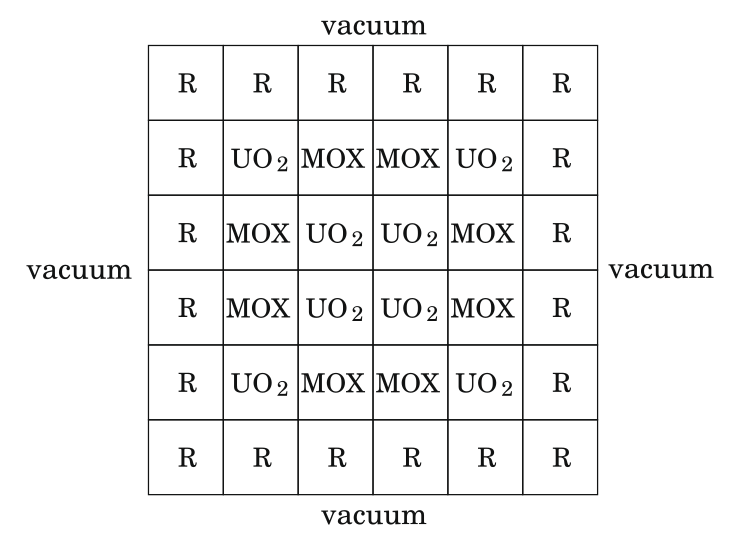
\includegraphics[width=0.45\textwidth]{../C5G2-benchmark/bench-config}
    \caption{2-D C5 MOX benchmark configuration. Image reproduced from \cite{capilla_applications_2009}. $R$ represents the reflectors.}
    \label{res:2d-bench-config1}
\end{figure}

\begin{figure}[htbp!]
    \centering
    \subfigure[UO$_2$ assembly.]{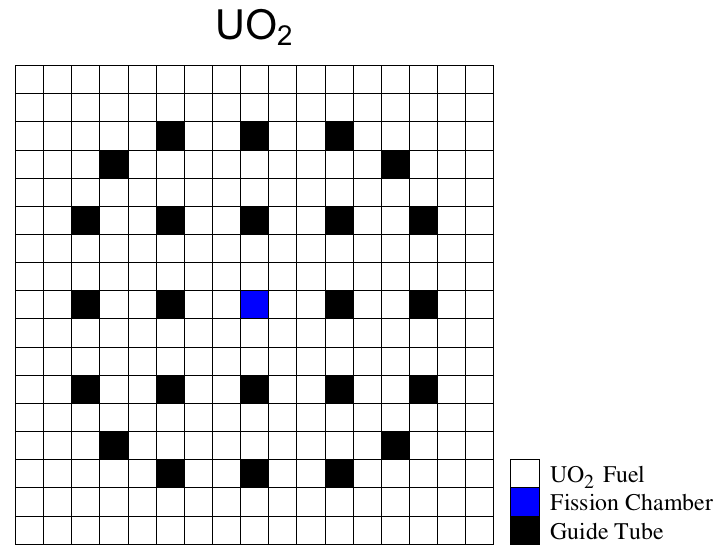
\includegraphics[width=0.45\textwidth]{../C5G2-benchmark/bench-config2}}
    \subfigure[MOX assembly.]{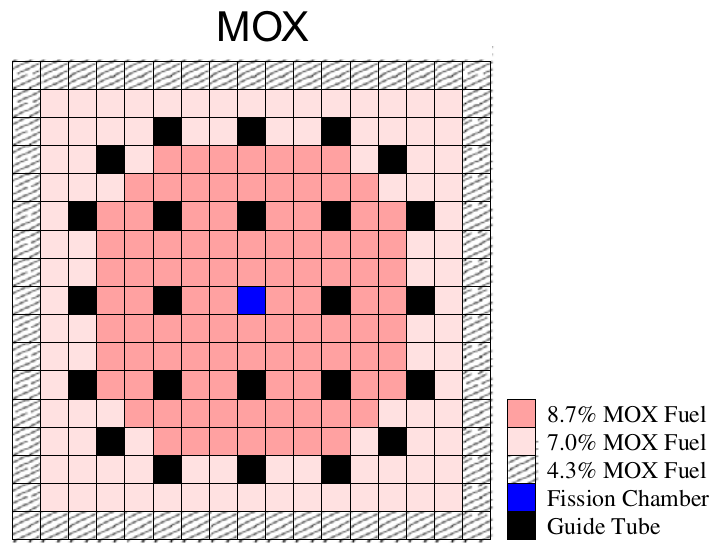
\includegraphics[width=0.45\textwidth]{../C5G2-benchmark/bench-config3}}
    \caption{Structure of the UO$_2$ and MOX assemblies. Images reproduced from \cite{capilla_applications_2009}.}
    \label{res:2d-bench-config2}
\end{figure}

\begin{table}[htbp!]
\centering
\caption{Two-group cross-sections [$cm^{-1}$] for the heterogeneous problem.}
\begin{tabular}{lccccc}
\toprule
Pin cell type & Group & $\Sigma_t$ & $\nu \Sigma_f$ & $\Sigma_{s0, 1 \rightarrow g}$ & $\Sigma_{s0, 2 \rightarrow g}$ \\
\midrule
4.3\% MOX       & 1     & 0.550      & 0.0075         & 0.520                         & 0.000                         \\
                & 2     & 1.100      & 0.3000         & 0.015                         & 0.900                         \\

7.0\% MOX       & 1     & 0.550      & 0.0075         & 0.520                         & 0.000                         \\
                & 2     & 1.010      & 0.3750         & 0.015                         & 0.760                         \\

8.7\% MOX       & 1     & 0.550      & 0.0075         & 0.520                         & 0.000                         \\
                & 2     & 1.060      & 0.4500         & 0.015                         & 0.760                         \\

UO$_2$          & 1     & 0.570      & 0.0050         & 0.540                         & 0.000                         \\
                & 2     & 1.100      & 0.1250         & 0.020                         & 1.000                         \\

Guide tube      & 1     & 0.586      & 0.0000         & 0.560                         & 0.000                         \\
                & 2     & 1.220      & 0.0000         & 0.025                         & 1.200                         \\

Reflector       & 1     & 0.611      & 0.0000         & 0.560                         & 0.000                         \\
                & 2     & 2.340      & 0.0000         & 0.050                         & 2.300                         \\

Fission chamber & 1     & 0.586      & $10^{-7}$      & 0.560                         & 0.000                         \\
                & 2     & 1.220      & 3 $\times 10^{-6}$   & 0.025                   & 1.200                         \\
\bottomrule
\end{tabular}
\label{tab:bench-xs-het}
\end{table}

\begin{table}[htbp!]
\centering
\caption{Two-group cross-sections [$cm^{-1}$] for the heterogeneous problem.}
\begin{tabular}{lccccc}
\toprule
Pin cell type & Group & $\Sigma_t$ & $\nu \Sigma_f$ & $\Sigma_{s0, 1 \rightarrow g}$ & $\Sigma_{s0, 2 \rightarrow g}$ \\
\midrule
MOX       & 1     & 0.560749      & 0.006952     & 0.530682     & 0.000000                     \\
          & 2     & 1.064663      & 0.339038     & 0.016025     & 0.836469                     \\

UO$_2$    & 1     & 0.573135      & 0.004589     & 0.543383     & 0.000000                     \\
          & 2     & 1.110761      & 0.113071     & 0.020463     & 1.018406                     \\

\bottomrule
\end{tabular}
\label{tab:bench-xs-hom}
\end{table}


\section{Results}

This sections presents the results for the one-dimensional (1-D) and two-dimensional (2-D) models.

\subsection{1-D test case}
\label{sec:results1d}

Figure \ref{res:1d-fixed} displays the neutron flux for one and three energy groups for a fixed source case.
Figure \ref{res:1d-crit} shows the neutron flux for one and three energy groups for an eigenvalue problem.
Table \ref{tab:1d-keff} compares the eigenvalue obtained with the SP3 and the diffusion solvers by calculating their difference with the formula
\begin{align}
  & \Delta_\rho = \left| \rho_{SP_3} - \rho_{Ref} \right| = \left| \frac{k_{SP_3}-1}{k_{SP_3}} - \frac{k_{Ref}-1}{k_{Ref}} \right| = \left| \frac{k_{SP_3}-k_{Ref}}{k_{SP_3} k_{Ref}} \right| \label{eq:delta-rho} \\
  \intertext{where}
  & k_{SP_3} = \mbox{eigenvalue obtained with SP3 solver} [-] \notag \\
  & k_{Ref} = \mbox{eigenvalue obtained with diffusion solver} [-]. \notag
\end{align}

% Fixed source
\begin{figure}[htbp!]
    \centering
    \subfigure[1 group.]{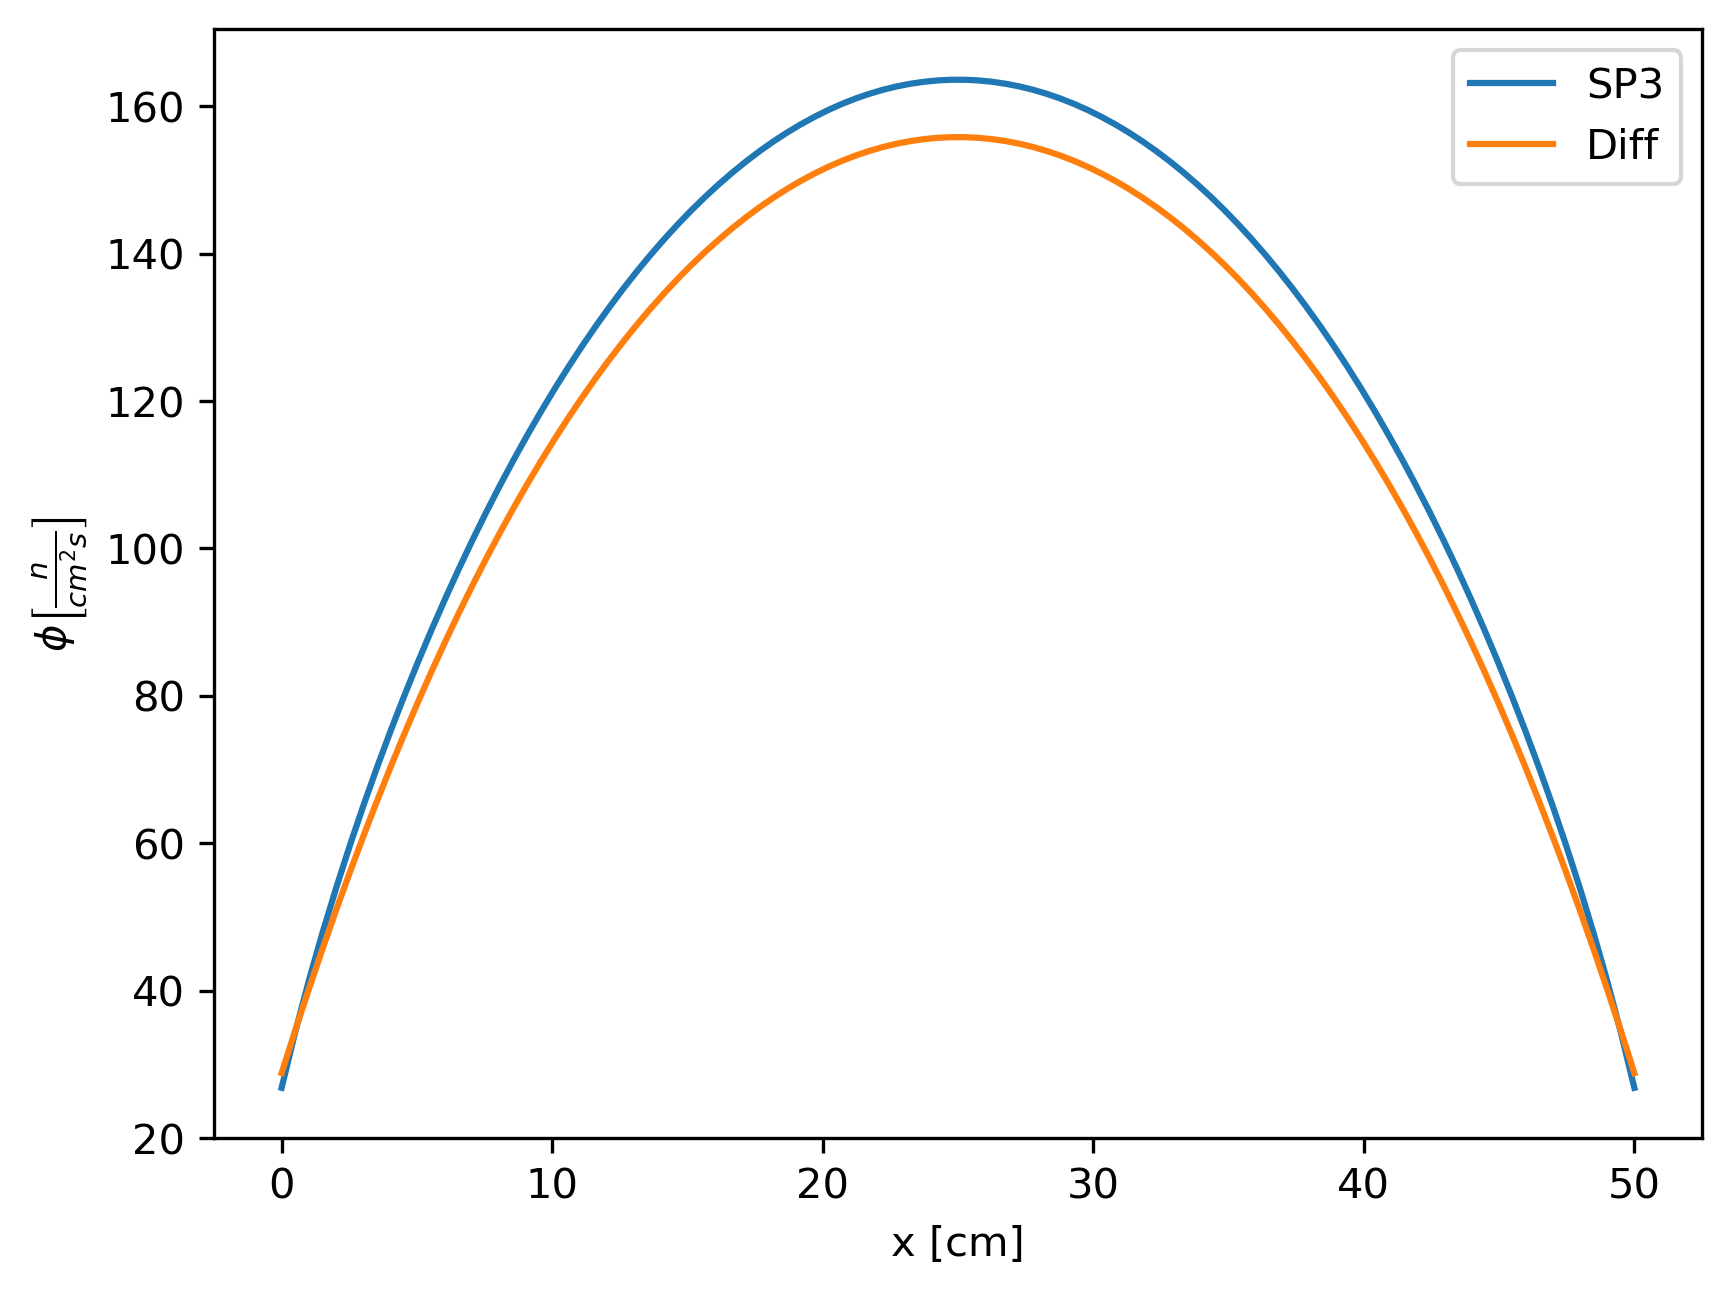
\includegraphics[width=0.45\textwidth]{../sp3-diffusion/output-1g-fixed}}
    \subfigure[3 groups.]{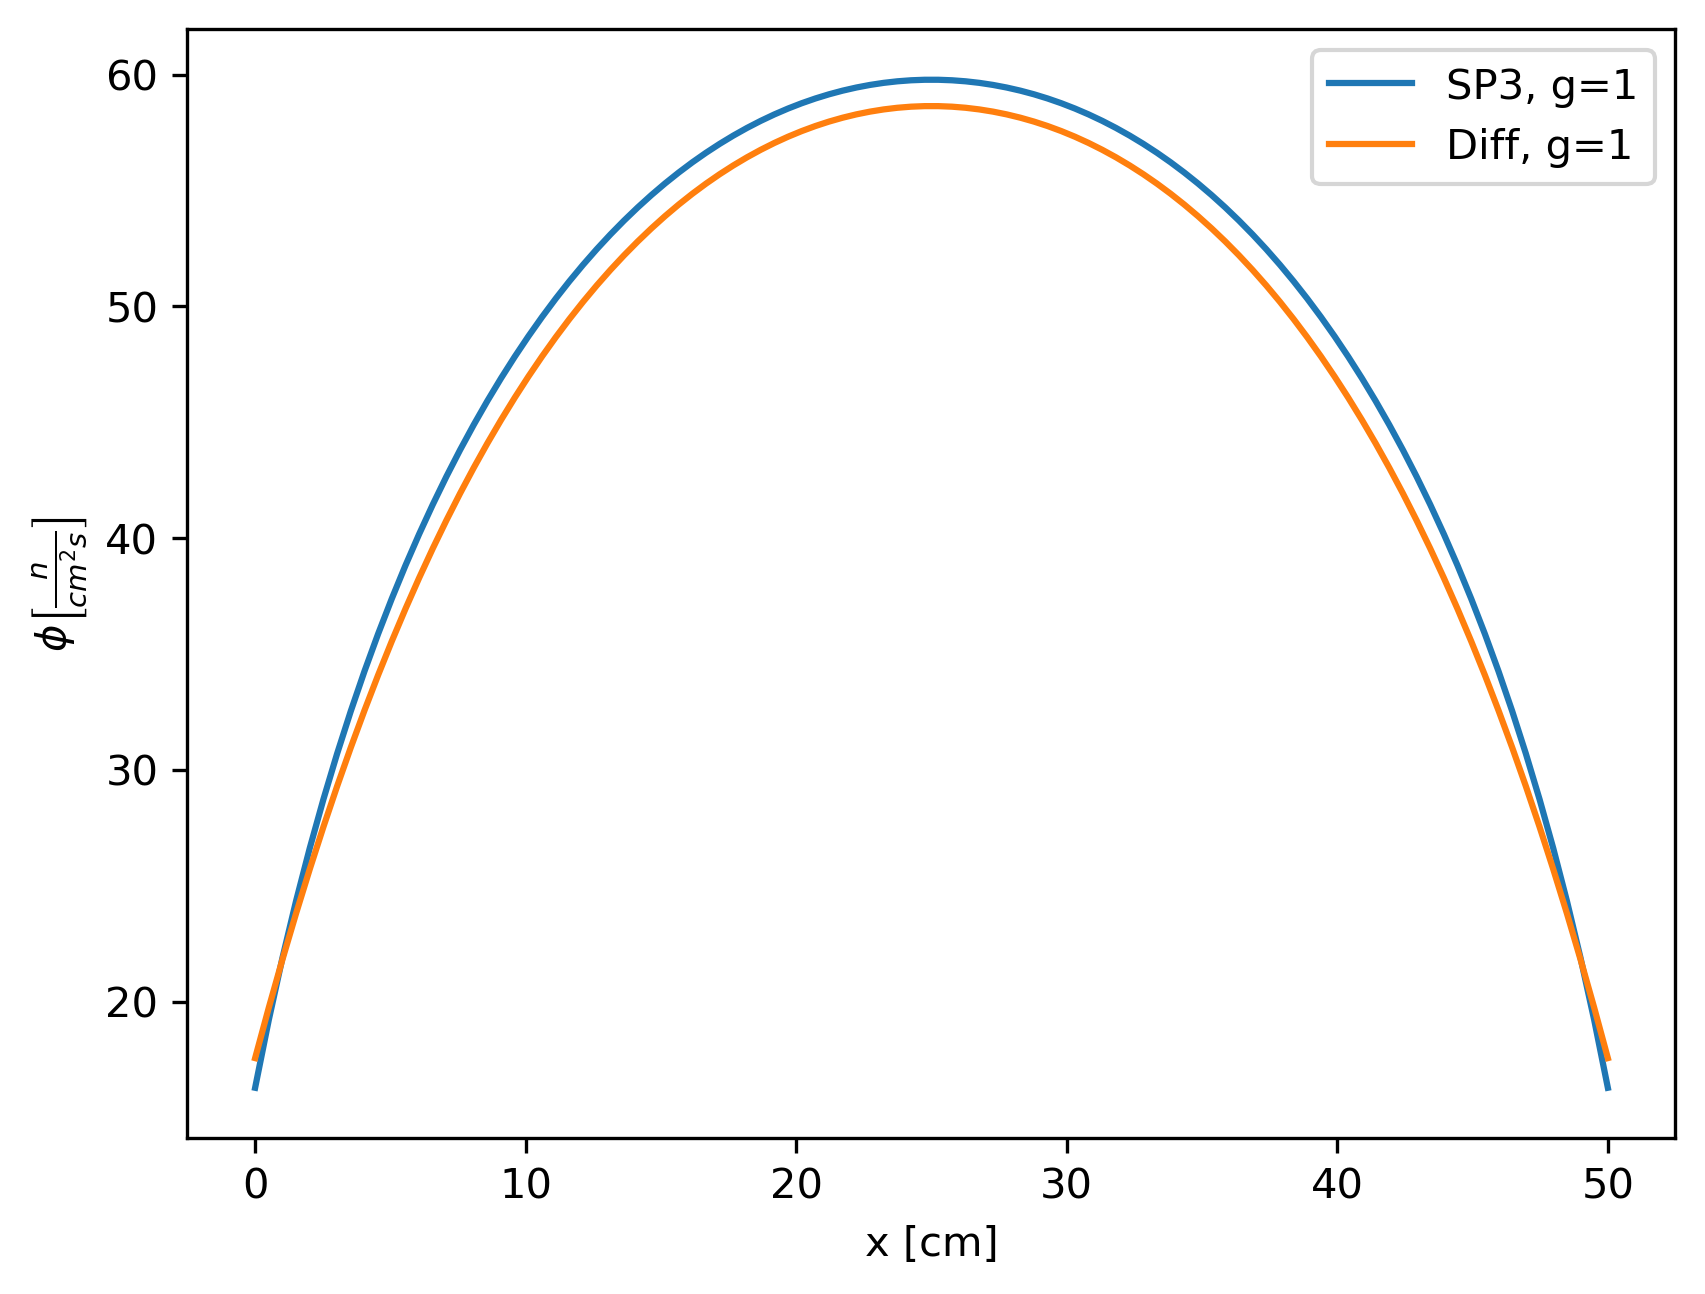
\includegraphics[width=0.45\textwidth]{../sp3-diffusion/output-3g-fixed}}
    \caption{Comparison of the scalar flux obtained with the SP3 and diffusion solvers for the fixed source case.}
    \label{res:1d-fixed}
\end{figure}

% Criticality source
\begin{figure}[htbp!]
    \centering
    \subfigure[1 group.]{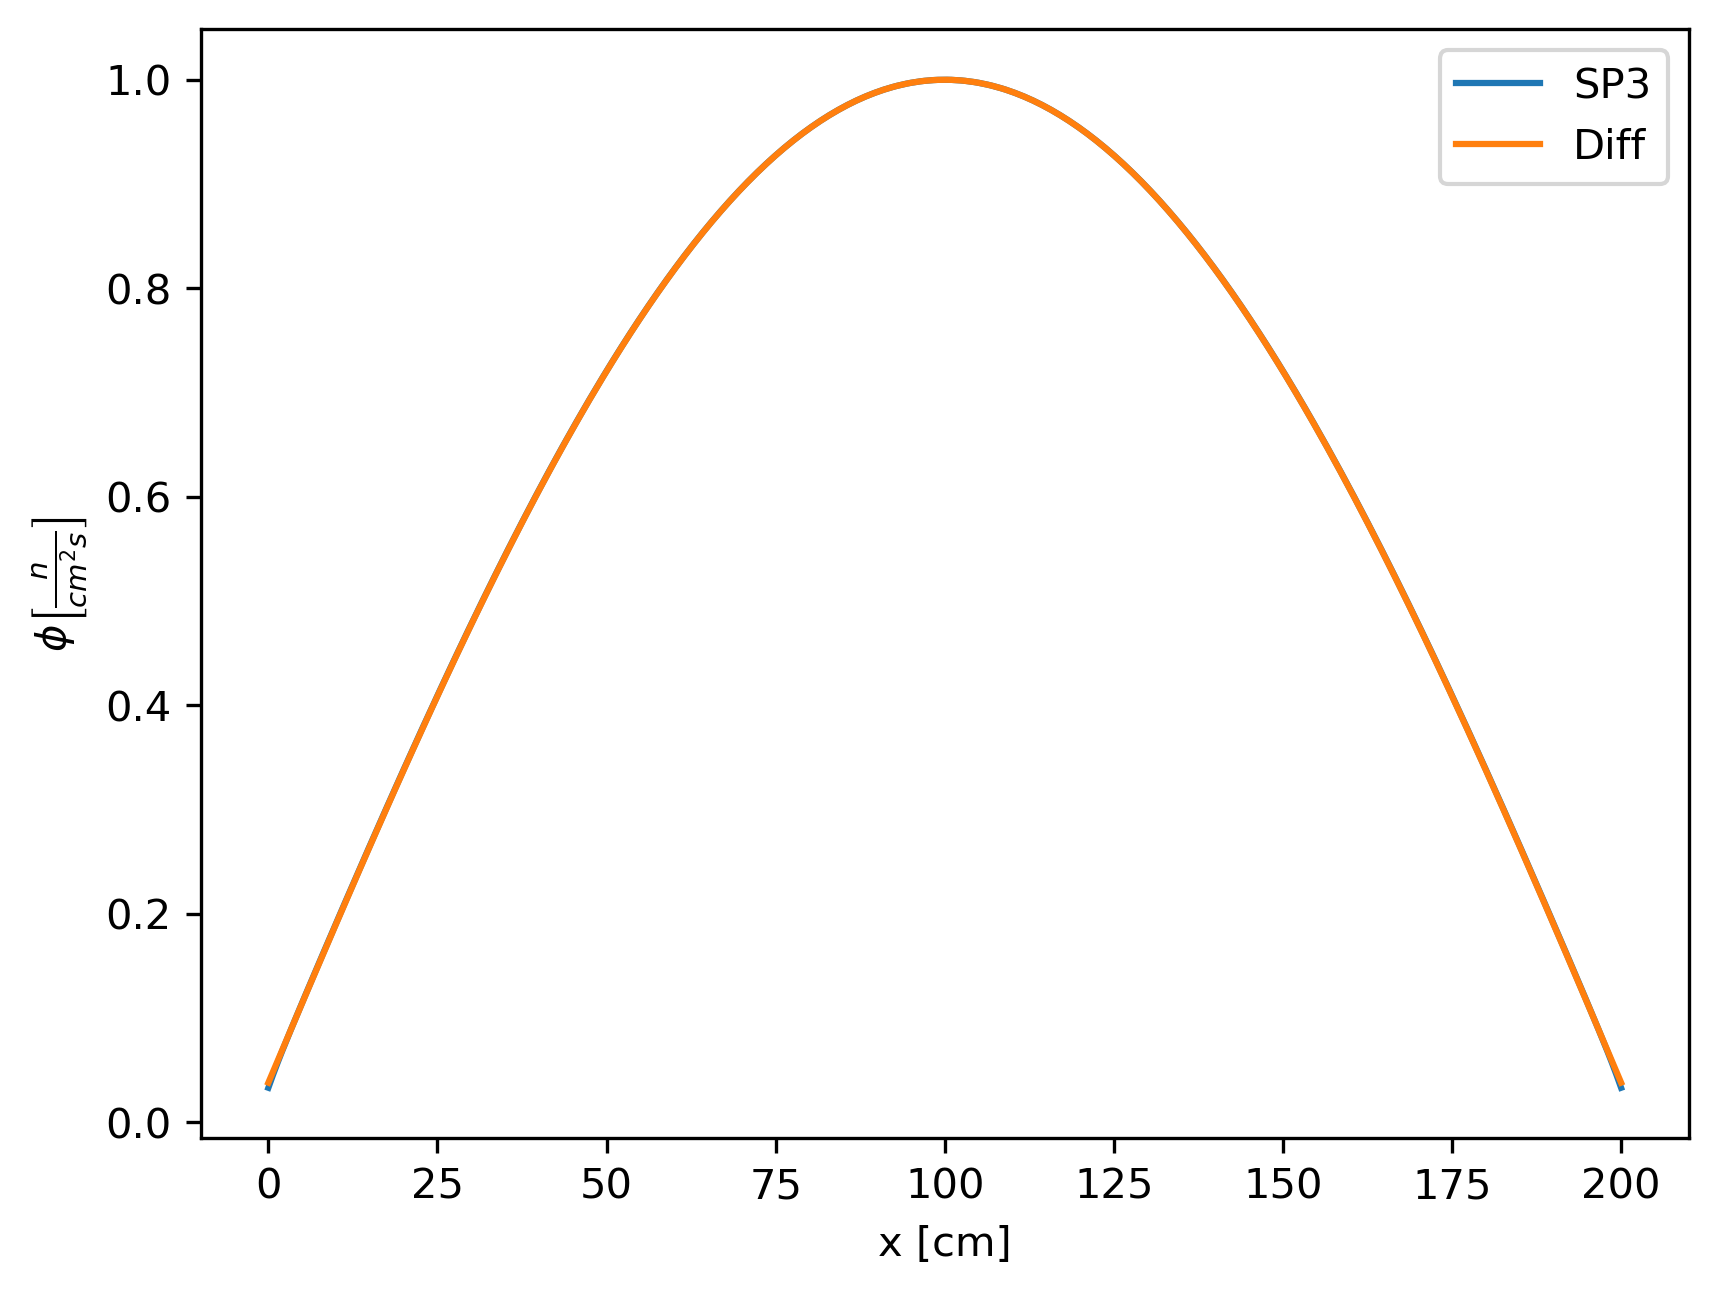
\includegraphics[width=0.45\textwidth]{../sp3-diffusion/output-1g-crit}}
    \subfigure[3 groups.]{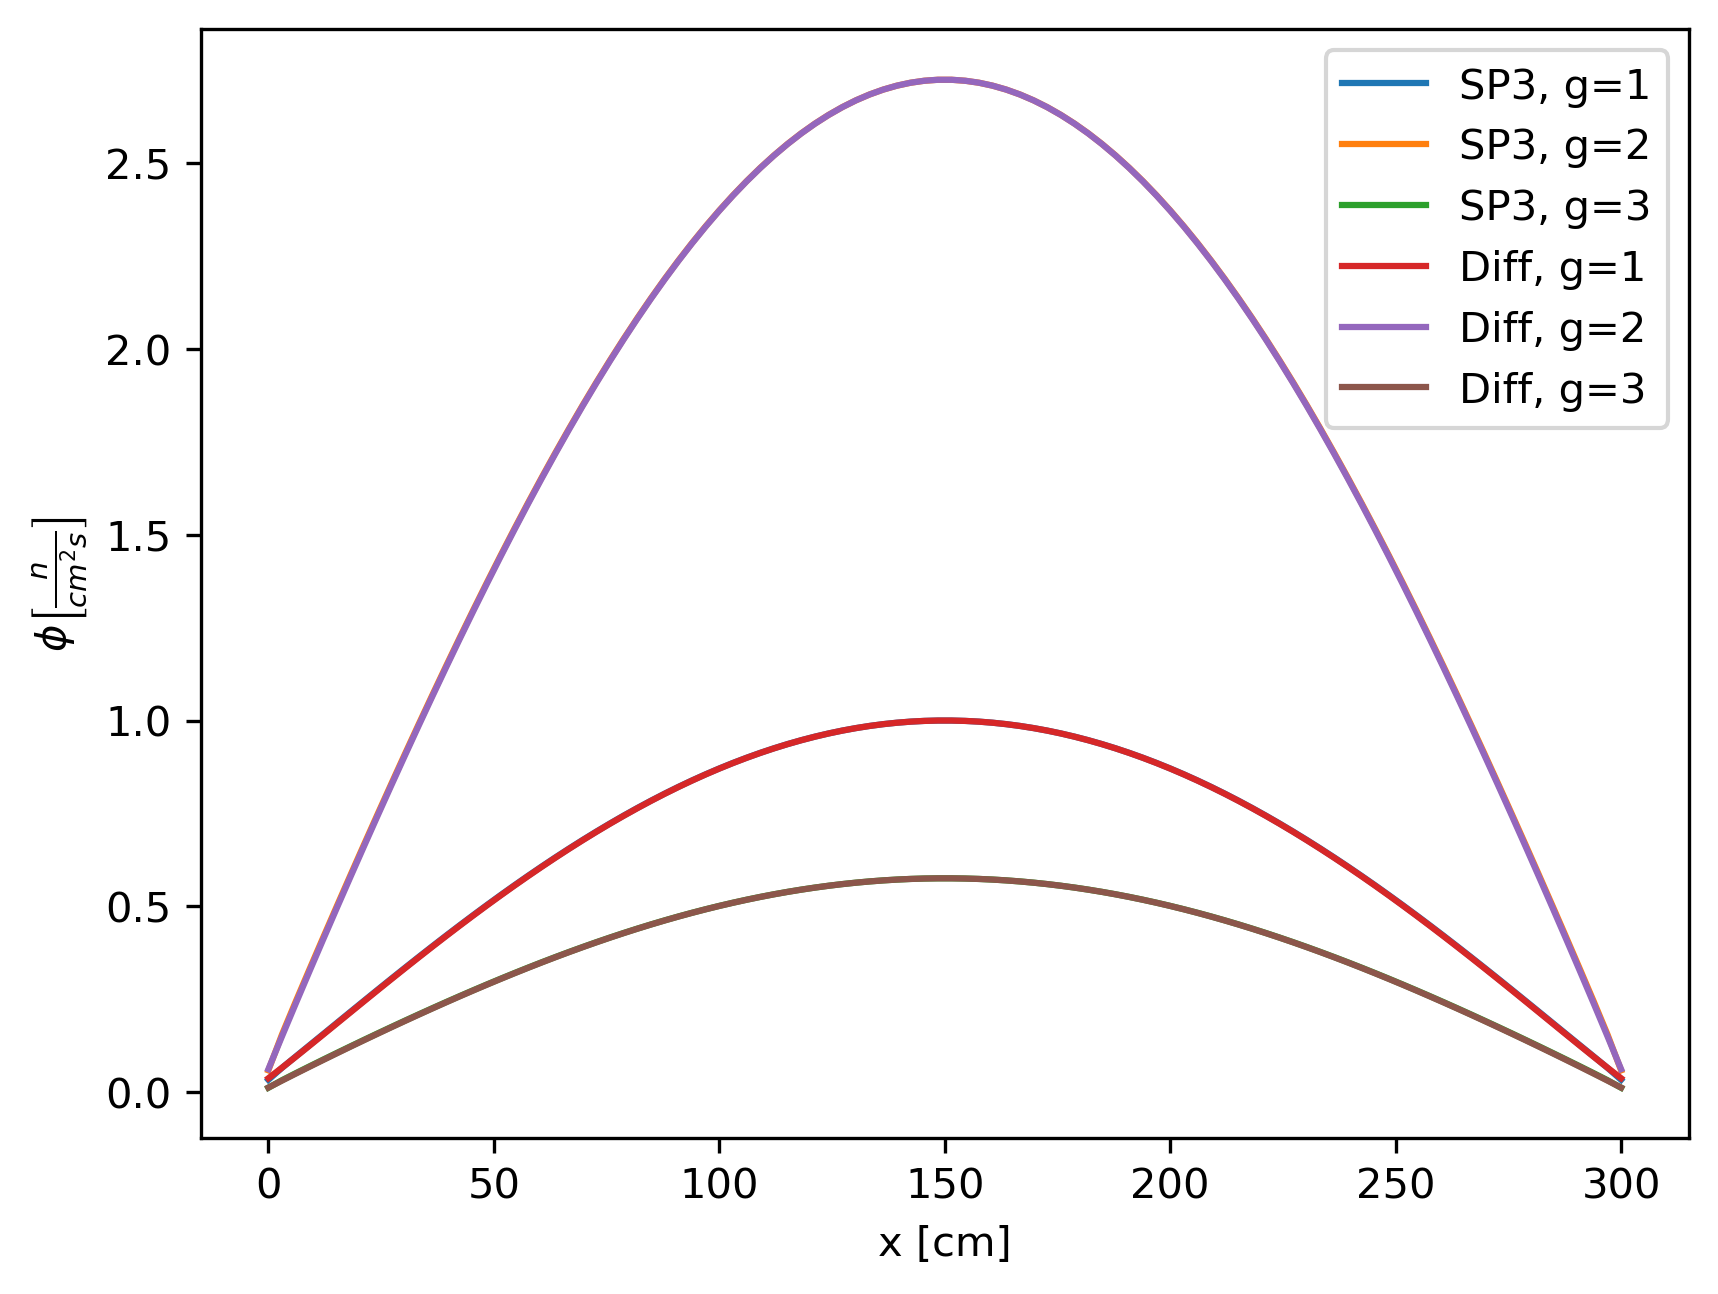
\includegraphics[width=0.45\textwidth]{../sp3-diffusion/output-3g-crit}}
    \caption{Comparison of the scalar flux obtained with the SP3 and diffusion solvers for the eigenvalues problem.}
    \label{res:1d-crit}
\end{figure}

% \usepackage{multirow}
\begin{table}[htbp!]
\centering
\caption{Comparison between the eigenvalue obtained with the SP3 and diffusion solvers.}
\begin{tabular}{ccccccc}
\toprule
 & Moltres      & \multicolumn{2}{c}{SP3}          \\
\midrule 
Number of groups & $k_{Ref}$    & $k_{SP_3}$ & $\Delta_\rho$ [pcm] \\
\midrule
1 & 1.05278     & 1.06004   & 650 \\
3 & 1.02878     & 1.03005   & 120 \\
\bottomrule
\end{tabular}
\label{tab:1d-keff}
\end{table}

\subsection{2-D test case}
\label{sec:results2d}

Figure \ref{res:2d-bench} displays the scalar flux of the C5G2 MOX Benchmark.
Table \ref{tab:2d-keff} compares the eigenvalue obtained with the SP3 solver ($k_{P_3}$) and the results in \cite{capilla_applications_2009} ($k_{Ref}$) by using equation \ref{eq:delta-rho}.

\begin{figure}[h!]
    \centering
    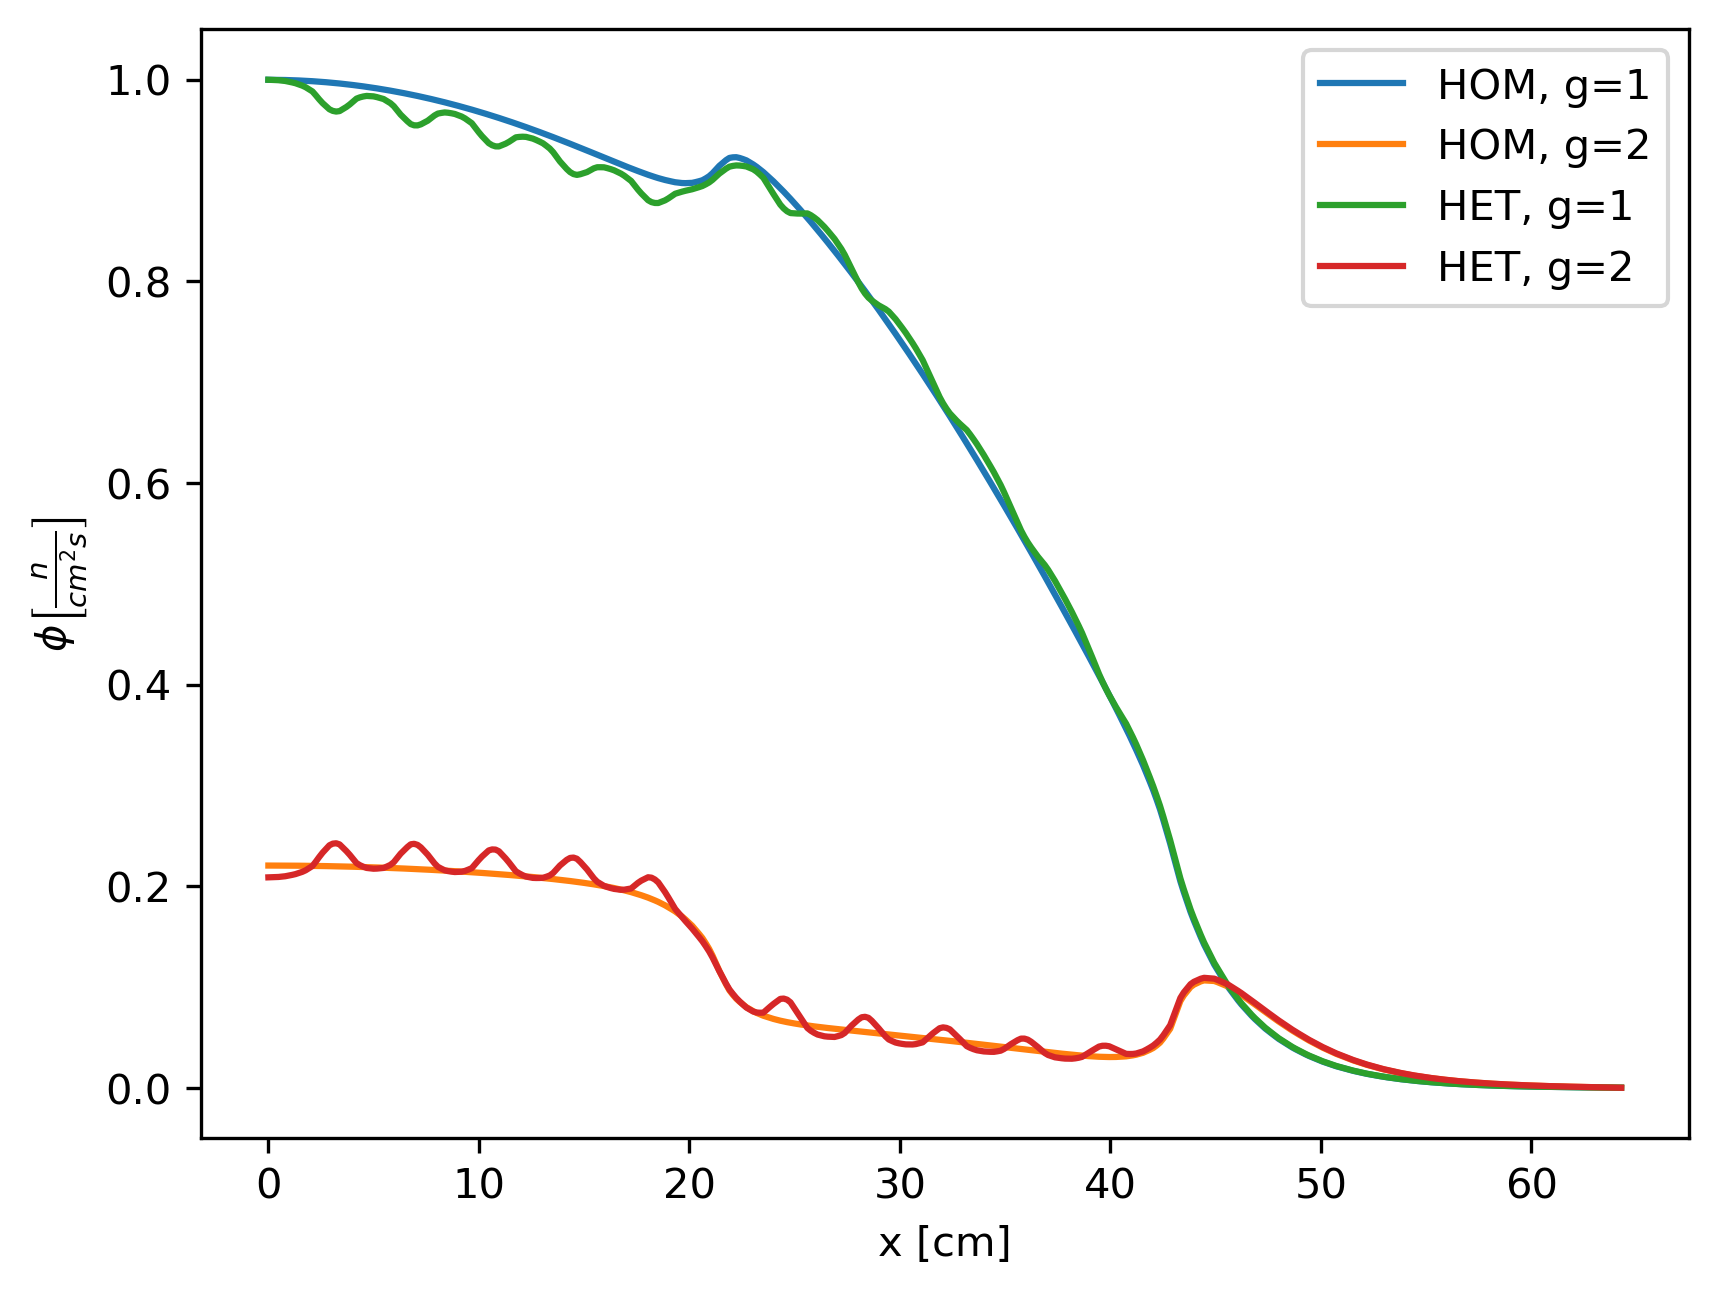
\includegraphics[width=0.45\textwidth]{../C5G2-benchmark/output-2g}
    \caption{Scalar flux on line between points (0, 10.71) and (64.26, 10.71). HOM: homogeneous case, HET: heterogeneous case.}
    \label{res:2d-bench}
\end{figure}

% \usepackage{multirow}
\begin{table}[htbp!]
\centering
\caption{Comparison between the eigenvalue obtained with the SP3 solver and the results in \cite{capilla_applications_2009}.}
\begin{tabular}{lccc}
\toprule
 & C5G2 Benchmark      & \multicolumn{2}{c}{SP3}          \\
\midrule
Case & $k_{Ref}$       & $k_{SP_3}$ & $\Delta_\rho$ [pcm] \\
\midrule
Heterogeneous & 0.96969  & 0.97106  & 145  \\
Homogeneous   & 0.96983  & 0.97061  &  83  \\
\bottomrule
\end{tabular}
\label{tab:2d-keff}
\end{table}

\section{Conclusions}

Section \ref{sec:results2d} results seem to indicate that the implementation of the $SP_3$ equations in a MOOSE-based application is correct.
On the other hand, the results from Section \ref{sec:results1d} show that the solution of the $SP_3$ equations yield very similar scalar fluxes to the diffusion equations.
While the diffusion solver calculates the flux with only one equation for each group, the $SP_3$ equations use two.
These characteristics would indicate that the diffusion solver is preferable over the $SP_3$ solver, yielding similar results by using less degrees of freedom to solve a problem.

\clearpage
\bibliographystyle{ieeetr}
\bibliography{bibliography}
\end{document}
